\section*{Лекция 13 (12.05)}

\begin{definition}
    $f : X \to \R, M \subset X$
    $x_0 \in M$ --- точка локального минимума $f $ на M, если $\exists \varepsilon > 0 : f(x_0) \leqslant f(x) \forall x \in B_{\varepsilon} (x_0) \cap M$.

\end{definition}



\tikzset{every picture/.style={line width=0.75pt}} %set default line width to 0.75pt        

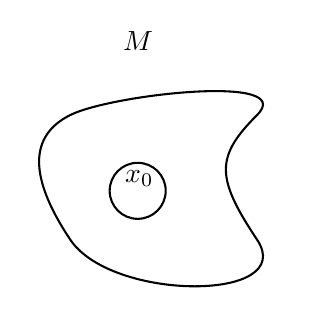
\begin{tikzpicture}[x=0.75pt,y=0.75pt,yscale=-1,xscale=1]
%uncomment if require: \path (0,300); %set diagram left start at 0, and has height of 300

%Shape: Polygon Curved [id:ds6019959986645902] 
\draw   (97,142) .. controls (117,132) and (207,122) .. (187,142) .. controls (167,162) and (167,172) .. (187,202) .. controls (207,232) and (117,232) .. (97,202) .. controls (77,172) and (77,152) .. (97,142) -- cycle ;
%Shape: Circle [id:dp7583149099046497] 
\draw   (116,178.5) .. controls (116,171.04) and (122.04,165) .. (129.5,165) .. controls (136.96,165) and (143,171.04) .. (143,178.5) .. controls (143,185.96) and (136.96,192) .. (129.5,192) .. controls (122.04,192) and (116,185.96) .. (116,178.5) -- cycle ;

% Text Node
\draw (121,100.4) node [anchor=north west][inner sep=0.75pt]    {$M$};
% Text Node
\draw (122,167.4) node [anchor=north west][inner sep=0.75pt]    {$x_{0}$};


\end{tikzpicture}

\begin{remark}
    Часто множество M задается условием, например $M$ --- множество уравнений некоторой функции, т.е. $\Phi : X \to \R, M = \{x \in X: \Phi(x) = 0\}$ (или что-то другое).
\end{remark}

Рассмотрим $f : \R ^ {m + n} \to \R, \Phi : z \in \R ^ {m + n} \to \R ^ m$

$M = \{ \Phi(z) = 0 \}$, $z \in M \Leftrightarrow \begin{cases}
    \Phi_1(z_1, \cdots, z_{m + n}) = 0\\
    \vdots\\
    \Phi_m(z_1, \cdots, z_{m + n}) = 0
\end{cases}$

\[
    d\Phi(z) = 
    \begin{pmatrix}
        \frac{\partial \Phi_j}{\partial z_k}
    \end{pmatrix} : \R ^ {m + n} \to \R ^ m
\]


$M $ невырождена в $(\cdot) z$ $\Leftrightarrow rank{\ d \Phi(z)} = m \hence$ выберем $m$ линейно независимых столбцов, переставим их в конец и переименуем переменные.

$z = (x_1, \cdots, x_n, y_1, ..., y_m)$

$d \Phi(x, y) = \begin{pmatrix}
    \underbrace{\partial_x \Phi(x, y)}_{n} &\bigg | & \underbrace{\partial_y \Phi(x, y)}_{m} 
\end{pmatrix}, \exists (\partial y \Phi(x, y)^ {-1})$

$\hence $ в окрестности точки имеем график функции $y = \phi(x)$

$z_0$ --- точка условного локального минимума $\widetilde{f}(x) = f(x, \phi(x)) \hence$ у  $\widetilde{f}$ $x_0$ --- точка локального минимума $\hence d \widetilde{f} (x_0) = 0 \Leftrightarrow \partial_x f(x_0, \phi(x_0)) + \partial_y f(x_0, \phi(x_0)) d \phi(x_0) = 0$ получаем уравнение из n переменных.


Знаем, что $\Phi(x, \phi(x)) = 0 \Rightarrow \partial_x \Phi(x_0, \phi(x_0)) + \partial_y \Phi(x_0, \phi(x_0)) d \phi(x_0) = 0$

Для удобства дальше положим $y_0 = \phi(x_0)$

Тогда выразим $d \phi(x_0): d \phi(x_0) = - (\partial_y \Phi(x_0, y_0)) ^ {-1} \partial_x \Phi(x_0, y_0)$

Теперь подставим полученное $d \phi(x_0)$ в уравнение выше и получим систему:

\[
\begin{cases}
    \partial_x f(x_0, y_0) - \underbrace{\partial_y f(x_0, y_0) (\partial_y \Phi(x_0, y_0))^{-1}}_{ = \lambda = (\lambda_1, \cdots, \lambda_m)} \partial_x \Phi(x_0, y_0) = 0\\

    \Phi(x_0, y_0) = 0
\end{cases}
\]

Ниже объяснена размерность $\lambda$:

\[
    \begin{cases}
    \Phi : \R ^ n \times \R ^ m \to \R ^ m\\
    f : \R ^ n \times \R ^ m \to \R\\
   (\partial_y \Phi(z_0))^{-1} : \R^ m \to \R ^m\\
   \partial_y f(z_0) : \R^m \to \R
    \end{cases}
\]

И заметим, что $\partial_y f(x_0, y_0) - \lambda \partial_y \Phi(x_0, y_0) = 0$

Условие Лагранжа: 

\[
    \exists \lambda : 
    \begin{cases}
        df(z_0) - \lambda d\Phi(z_0) = 0 \text{ (m +n) уравнений} \\
        \Phi(z_0) = 0 \text{ (m) уравнений}
    \end{cases}
\]

число неизвестных: $2 m + n$

число уравнений: $2 m + n$

$\lambda$ --- неопределенные множители Лагранжа

\begin{theorem}
    Если $z_0$ --- точка условного локального экстремума $f$ при условии $\Phi = 0$ и $\Phi $ не вырождена в $(\cdot) z_0 \hence \exists \lambda = (\lambda_1, ..., \lambda_m)$ т.ч. $d(f - \lambda \Phi)(z_0) = 0 \Leftrightarrow d(f - \lambda_1 \Phi_1 - \cdots - \lambda_m \Phi_m)(z_0) = 0$. 
\end{theorem}


Геометрический (менее формальный) подход

Если смещаемся вдоль поверхности от $z_0$ в любом направлении $\hence$ значение должно расти.

Смещение по касательному вектору и по поверхности в окрестности должно быть похожим.

\quad

\tikzset{every picture/.style={line width=0.75pt}} %set default line width to 0.75pt        

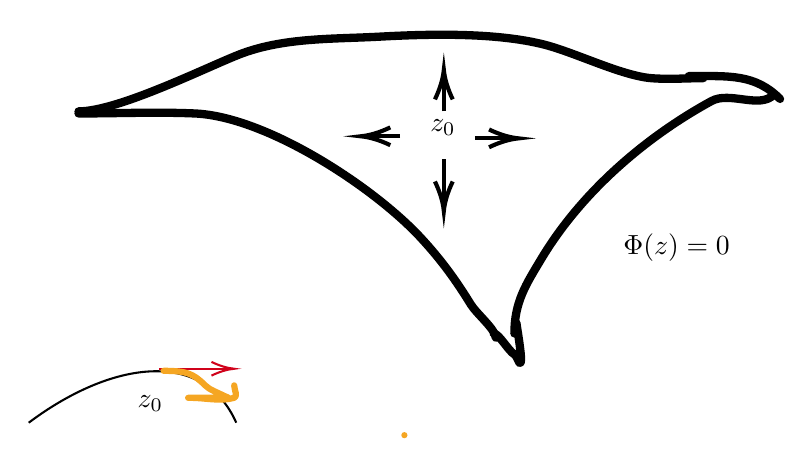
\begin{tikzpicture}[x=0.75pt,y=0.75pt,yscale=-1,xscale=1]
%uncomment if require: \path (0,300); %set diagram left start at 0, and has height of 300

%Shape: Free Drawing [id:dp6931486391064557] 
\draw  [line width=3] [line join = round][line cap = round] (72,112) .. controls (90.67,112) and (109.35,111.2) .. (128,112) .. controls (162.57,113.48) and (214.39,147.51) .. (237,172) .. controls (246.68,182.48) and (253.7,192.13) .. (261,204) .. controls (263.74,208.45) and (273,216.15) .. (273,220) ;
%Shape: Free Drawing [id:dp7064835250745065] 
\draw  [line width=3] [line join = round][line cap = round] (72,111) .. controls (91.71,111) and (136.64,88.25) .. (151,83) .. controls (171.81,75.39) and (194.87,76.2) .. (217,75) .. controls (238.8,73.82) and (272.95,72.67) .. (297,79) .. controls (311.69,82.87) and (333.9,93.86) .. (348,95) .. controls (356.31,95.67) and (364.67,95) .. (373,95) ;
%Shape: Free Drawing [id:dp23495454486814937] 
\draw  [line width=3] [line join = round][line cap = round] (282,218) .. controls (282,202.82) and (287.58,194.37) .. (295,182) .. controls (314.03,150.29) and (344.61,123.67) .. (377,106) .. controls (385.76,101.22) and (400.12,109.88) .. (407,103) ;
%Shape: Free Drawing [id:dp9617954244406846] 
\draw  [line width=3] [line join = round][line cap = round] (366,94) .. controls (385.55,94) and (397.85,92.85) .. (410,105) ;
%Straight Lines [id:da15312982675638276] 
\draw [color={rgb, 255:red, 0; green, 0; blue, 0 }  ,draw opacity=1 ][line width=1.5]    (248,111) -- (248,94) ;
\draw [shift={(248,91)}, rotate = 90] [color={rgb, 255:red, 0; green, 0; blue, 0 }  ,draw opacity=1 ][line width=1.5]    (14.21,-4.28) .. controls (9.04,-1.82) and (4.3,-0.39) .. (0,0) .. controls (4.3,0.39) and (9.04,1.82) .. (14.21,4.28)   ;
%Straight Lines [id:da6410064287473216] 
\draw [color={rgb, 255:red, 0; green, 0; blue, 0 }  ,draw opacity=1 ][line width=1.5]    (248,134) -- (248,156) ;
\draw [shift={(248,159)}, rotate = 270] [color={rgb, 255:red, 0; green, 0; blue, 0 }  ,draw opacity=1 ][line width=1.5]    (14.21,-4.28) .. controls (9.04,-1.82) and (4.3,-0.39) .. (0,0) .. controls (4.3,0.39) and (9.04,1.82) .. (14.21,4.28)   ;
%Straight Lines [id:da5996502583636397] 
\draw [color={rgb, 255:red, 0; green, 0; blue, 0 }  ,draw opacity=1 ][line width=1.5]    (263,124) -- (281,124) ;
\draw [shift={(284,124)}, rotate = 180] [color={rgb, 255:red, 0; green, 0; blue, 0 }  ,draw opacity=1 ][line width=1.5]    (14.21,-4.28) .. controls (9.04,-1.82) and (4.3,-0.39) .. (0,0) .. controls (4.3,0.39) and (9.04,1.82) .. (14.21,4.28)   ;
%Straight Lines [id:da45593982174276837] 
\draw [color={rgb, 255:red, 0; green, 0; blue, 0 }  ,draw opacity=1 ][line width=1.5]    (227,123) -- (211,123) ;
\draw [shift={(208,123)}, rotate = 360] [color={rgb, 255:red, 0; green, 0; blue, 0 }  ,draw opacity=1 ][line width=1.5]    (14.21,-4.28) .. controls (9.04,-1.82) and (4.3,-0.39) .. (0,0) .. controls (4.3,0.39) and (9.04,1.82) .. (14.21,4.28)   ;
%Shape: Free Drawing [id:dp934471589522585] 
\draw  [line width=3] [line join = round][line cap = round] (272,218) .. controls (274.57,218) and (279.2,226.6) .. (282,228) .. controls (283.49,228.75) and (284.25,233.49) .. (285,232) .. controls (285.96,230.08) and (283,214.01) .. (283,213) ;
%Curve Lines [id:da9829400721912698] 
\draw    (48,261) .. controls (88,231) and (132,225) .. (148,261) ;
%Straight Lines [id:da3012413224869941] 
\draw [color={rgb, 255:red, 208; green, 2; blue, 27 }  ,draw opacity=1 ]   (111,235) -- (145,235) ;
\draw [shift={(147,235)}, rotate = 180] [color={rgb, 255:red, 208; green, 2; blue, 27 }  ,draw opacity=1 ][line width=0.75]    (10.93,-3.29) .. controls (6.95,-1.4) and (3.31,-0.3) .. (0,0) .. controls (3.31,0.3) and (6.95,1.4) .. (10.93,3.29)   ;
%Shape: Free Drawing [id:dp6407520907737706] 
\draw  [color={rgb, 255:red, 245; green, 166; blue, 35 }  ,draw opacity=1 ][line width=2.25] [line join = round][line cap = round] (113,236) .. controls (123.85,236) and (127.16,237.16) .. (133,243) .. controls (135.43,245.43) and (139,246.33) .. (142,248) .. controls (142.65,248.36) and (144.75,249) .. (144,249) .. controls (138,249) and (120,249) .. (126,249) .. controls (133,249) and (140.27,250.92) .. (147,249) .. controls (148.92,248.45) and (147,245) .. (147,243) ;
%Shape: Free Drawing [id:dp8324402414283608] 
\draw  [color={rgb, 255:red, 245; green, 166; blue, 35 }  ,draw opacity=1 ][line width=2.25] [line join = round][line cap = round] (229,267) .. controls (229,267) and (229,267) .. (229,267) ;

% Text Node
\draw (240,113.4) node [anchor=north west][inner sep=0.75pt]    {$z_{0}$};
% Text Node
\draw (333,168.4) node [anchor=north west][inner sep=0.75pt]    {$\Phi ( z) =0$};
% Text Node
\draw (99,246.4) node [anchor=north west][inner sep=0.75pt]    {$z_{0}$};


\end{tikzpicture}

\quad

$df(z_0)h = 0$, если $h$ касательный к поверхности $\{ \Phi = 0 \}$ $\Leftrightarrow \langle \nabla \Phi(z_0), h \rangle = 0$

Если $\nabla \Phi \perp h \hence \nabla f \perp h$

\begin{enumerate}
    \item $\Phi = \Phi_1$, $h \in T_{z_0} M \leftrightarrow h \perp \nabla \Phi(z_0)$
    \item $\Phi = (\Phi_1, ..., \Phi_m)$, $h \in T_{z_0}M \leftrightarrow h \perp span(\nabla \phi_1(z_0), ..., \nabla \phi_m(z_0)) = L$
    
    $\forall h \perp L, \nabla f(z_0) \perp h \hence \nabla f (z_0) \in L \hence \exists \lambda_1, \cdots, \lambda_m : \nabla f(z_0) = \lambda_1 \nabla \Phi_1(z_0) + \cdots + \lambda_m \nabla \Phi_m(z_0)$.
\end{enumerate}

\begin{example}
    (минимум квадратичной формы на сфере)

    $\R ^ m, f(x) = \langle Ax, x \rangle$, А - симметричная матрица

    $S = S ^ {m - 1} \subset \R ^ m = \{ x : \norm{x}_2 = 1 \}, f \underset{x \in S}{\to}min$

    $\Phi(x_1, \cdots, x_m) = x_1 ^ 2 + \cdots x_m ^ 2 - 1 $

    В точке минимума $\exists \lambda \in \R : d(f - \lambda \Phi)(x) = 0$

    $df(x) = \langle A dx, x \rangle + \langle Ax, dx \rangle = 2 \langle Ax, dx \rangle$

    $d\Phi (x) = 2 \langle x, dx \rangle$

    $Ax = \lambda x \hence x $ --- с.в. $A$, $\lambda$ --- с.ч.

    $\frac{\partial f}{\partial x_j} - \lambda \frac{\partial \phi}{\partial x_j} = 0 = 2 (\sum a_{i,j}x_i - \lambda x_j) = Ax = \lambda x$

    Нашли $\lambda_1, v_1$
    
    $x \perp v_1 \hence Ax \perp v_1$

    $\langle Ax, v_1 \rangle = \langle x, A v_1 \rangle = \lambda_1 \langle x, v_1 \rangle = 0$

    $A_1, f_1, \cdots$ действуют на $\{ v_1 \} ^ {\perp}$
    
    $A_1 = A \bigg |_{v_1 ^ \perp }, f_1 = f \bigg | _{{v_1}^{\perp}}$

    $\min \limits_{\Phi(x) = 0, x \perp v_1} f_1$ $\longrightarrow$ получаем второе по величине с.ч. и с.в. и т.д.
\end{example}


\begin{example} (Задача Дидона)




\tikzset{every picture/.style={line width=0.75pt}} %set default line width to 0.75pt        

\begin{tikzpicture}[x=0.75pt,y=0.75pt,yscale=-1,xscale=1]
%uncomment if require: \path (0,300); %set diagram left start at 0, and has height of 300

%Straight Lines [id:da3576862247295107] 
\draw    (175,183) -- (367,183) ;
%Curve Lines [id:da4447152855498784] 
\draw    (203,180) .. controls (243,150) and (282,140) .. (303,180) ;

% Text Node
\draw (191,200.4) node [anchor=north west][inner sep=0.75pt]    {$0$};
% Text Node
\draw (306,209.4) node [anchor=north west][inner sep=0.75pt]    {$1$};
% Text Node
\draw (272,119.4) node [anchor=north west][inner sep=0.75pt]    {$f$};


\end{tikzpicture}

Хотим максимизировать площадь под графиком, фиксируя длину.

\[
    J[F] = \int_0^1 f(x) dx \to \max
\]

\[
    f(0) = f(1) = 0
\]

\[
    \Phi[f] = \int_0^1 \sqrt{1 + (f')^2} dx - l = 0
\]

\[
    L = \{ f \in C^2 [0, 1] |\, f(0) = f(1) = 0 \}
\]

\underline{Метод множителей Лагранжа: } 

$\exists \lambda$ т.ч. $\forall h : h(0) = h(1) = 0, \partial_h(J - \lambda \Phi)(f) = 0$. То есть производная по всем направлениям равна 0.

\begin{proof}

Предположим, что $\exists h_0 : \partial h_0 \Phi(f) \neq 0$


Выбрали h, положим $g(t, s) = \Phi[f + th + sh_0]$

И хотим найти $s : g(t, s) = 0$

Цель: $\exists s(t) : g(t, s(t)) = 0$

$\partial_s g(t, s) = \partial_{h_0} \Phi(f + th + sh_0) $

Т.к. $\exists (\partial_s g(0, 0)) ^ {-1} = (\partial_{h_0} \Phi (f)) ^ {-1}$, то:

Тогда по теореме о неявной функии $\exists s(t) : (\star) = \Phi(f + th + s(t)h_0) = 0$

Давайте тогда заведем еще одну функцию: $\phi(t) = J(f + th + s(t)h_0) \hence$ 0 --- точка локального максимума(т.к. мы считаем, что $f$ точка локального максимума в $J$) $\hence \phi'(0) = 0$

Тогда распишем $\phi'(0) = \partial_h J(f) + s'(0) \partial _{h_0} J(f) = 0$

И при $t = 0 \Rightarrow \dfrac d {dt} (\star) = \dfrac {d\Phi} {dt} (f + th + s(t)h_0) = \partial_h \Phi(f) + s'(0) \partial_{h_0} \Phi(f) = 0$

Теперь выразим $s'(0)$ и подставим в верхнее равенство: $\partial_h J(f) - \underbrace{\frac{\partial h_0 J(f)}{\partial h_0 \Phi(f)}}_{= \lambda} \partial_h \Phi(f) = 0$

Тогда $\forall h \Rightarrow \partial_h (J - \lambda \Phi)(f) = 0$

\end{proof}

\[
    (J - \lambda \Phi)(f) = \int_0^1 \underbrace{f - \lambda \sqrt{1 + (f') ^ 2} dx}_{F(x, f, f')}
\]

По уравнению Эйлера-Лагранжа: $\partial_2 F (...) - \frac{d}{dx} \partial_3 F (...) = 0$. То есть мы минимизируем функционал, чтобы выполнилась теорема сверху.

Тогда получим:

\[
    1 - \frac{d}{dx} \left(-\lambda \frac{f'}{\sqrt{1 + (f')^2}}\right) = 0 \Rightarrow -\lambda \frac{f'}{\sqrt{1 + (f') ^ 2}} = x + c
\]

Выразим $f'$:

\[
    \Leftrightarrow \frac{f'}{\sqrt{1 + (f') ^ 2}} = -\frac{(x + c)}{\lambda} \Leftrightarrow \frac{(f') ^ 2}{1 + (f') ^ 2} = \frac{(x + c) ^ 2}{\lambda ^ 2} \Leftrightarrow
\]

\[
    \Leftrightarrow \frac{1}{(f') ^ 2} = \frac{\lambda ^ 2}{(x + c) ^ 2} - 1 \Leftrightarrow f'(x) = \sqrt{\frac{(x + c) ^ 2}{\lambda ^ 2 - (x + c) ^ 2}} \Leftrightarrow
\]

\[
    \Leftrightarrow f(x) = \bigint \sqrt{\frac{(x + c) ^ 2}{x ^ 2 - (x + c) ^ 2}} dx \Leftrightarrow f = -\sqrt{\lambda^2 - (x + c)^2} + c_1
\]

Возьмем $\Rightarrow (f(x) - c_1) ^ 2 + (x + c) ^ 2 = \lambda ^ 2$. Получили график окружности, осталось выполнить все условия.
\end{example}
